
\section{Wrapper}\label{sec:Wrapper}

\subsubsection*{Context} You are part of an active, long-running, and possibly quite complex project with more than a handful of participants.  How do you manage?
\textbf{The project presents a certain user interface to the world.  If the primary interface is based on a simple leader/follower dichotomy, then it's easy to know where everyone stands.  But peeragogy requires a more sophisticated facilitation/colearning dynamic.}

\subsubsection*{Problem} In an active project, it can be effectively impossible to stay up to date with all of the details.  Not everyone will be able to attend every meeting (see \patternname{Heartbeat}) or read every email.  Project participants can easily get lost and drift away.  The experience can be much more difficult for \patternnameplural{Newcomer}: joining an existing project can feel like trying to climb aboard a rapidly moving vehicle.  If you've taken time off, you may feel like things have moved on so far that you cannot catch up.  Information overload is not the only concern: there is also a problem with missing information.  If they aren't shared, key skills can quickly become bottlenecks (see \patternname{Carrying capacity}).

\subsubsection*{Solution}
% DK: Be more direct.  Don’t say what “can” be done…just say what to do. [also, typo -jc]
Someone involved with the project should regularly create a wrap-up summary, distinct from other project communications, that makes current activities comprehensible to people who may not have been following all of the details.  In addition, project members should keep other informative resources like the landing page, \patternname{Roadmap}, and documentation up to date.  Ensure that these resources accurately represent the facts on the ground, and check empirically to see if they really show interested parties how they can get involved.

\subsubsection*{Rationale}
According to the theory proposed by Yochai Benkler, for free/open ``commons-based'' projects to work, it is important for participants to the ability to contribute small pieces, and for the project to have a way to stitch those pieces together \cite{coases-penguin}.  The \patternname{Wrapper} helps perform this integrative stitching function.  If you value participation, you may have to do some serious work to facilitate access to process.

\subsubsection*{Resolution} 
% DK: This sounds like Rationale
Regularly circulated summaries can help to engage or re-engage members of a project, and can give an emotional boost to peeragogues who see their contributions and concerns mentioned.  Well-maintained records chronicle the project's history; up-to-date documentation makes the project more robust; a coherent look-and-feel makes it accessible.
%
In short, surfaces matter.  People can tell the difference between a project that is led by example and one that is led by fiat;
they can see right away if the project welcomes contributions with love, and if the participants feel they have something valuable to share.

\subsubsection*{Example 1} 
There many data streams around the Wikimedia project that comprise
an elaborate \patternname{Wrapper} function for the project, including
Today's Featured Article, appearing on the front page of
Wikipedia, as well as formal annual reports from the nonprofit.\footnote{\url{https://en.wikipedia.org/wiki/Wikipedia:Today\%27s_featured_article}}\textsuperscript{,}\footnote{\url{https://wikimediafoundation.org/wiki/Annual_Report}}
Inevitably, this can be improved to connect users to just the
information they are looking for.  Also, while citing Wikipedia itself
remains somewhat controversial, Wikipedia is often used as a
\patternname{Wrapper} for the scientific literature, that is, as a
first place to look for articles that can be cited.

\subsubsection*{Example 2} In-person meetings are no less relevant
for contemporary humans than they were a century ago, even though we
often work remotely, and have learned more about how to assemble on the fly
\cite{rheingold2007smart}.  Getting together for conventions, dance
parties, and commencement ceremonies could comprise an important part
of the future university's \patternname{Wrapper} function, even if
these events do not always take place in one specific Assembly Hall.

%\subsubsection*{Summary}


\begin{framed}
\noindent 
\emph{What's Next.}
We have prototyped and deployed a visual ``dashboard'' that people can use to get involved with the ongoing work in the project.  Let's improve it, and match it with an improved interaction design for peeragogy.org.
\end{framed}    


\begin{figure}
\begin{tikzpicture}[every node/.style={anchor=south west,inner sep=0pt},x=1mm, y=1mm,]
     \node (fig1) at (0,0)
       {\includegraphics[width=\textwidth,trim=0mm 135mm 0mm 0mm,clip=true]{figures/peeragogy_dashboard_draft1/peeragogy_dashboard_draft1.jpg}};
     \node (fig2) at (55, 14)
       {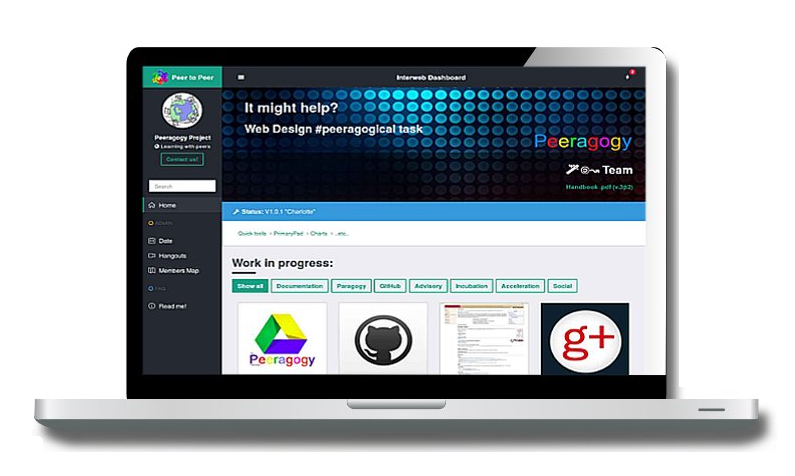
\includegraphics[width=.45\textwidth,trim=0mm 0mm 0mm 0mm,clip=true]{figures/dashboard/dash-trans.png}};  
\end{tikzpicture}
\caption{Design for a Peeragogy project dashboard (design sketch by Amanda Lyons, prototype by Fabrizio Terzi; images used with permission).\label{dashboard}}
\end{figure}

